\section{Introduction}

In recent years, \gls{IL}~\citep{schaal1999imitation, zare2024survey}, also often referred to as \gls{LFD} and, particularly, \gls{BC}, has gained significant momentum due to its sample and iteration efficiency in learning complex tasks, compared to alternatives such as \gls{RL}. The community has been focused on enhancing motion policies learned from demonstration to be more robust, high-performing, and generalizable by (i) integrating modern ML architectures like diffusion policies or flow matching to boost expressiveness and performance~\citep{chi2023diffusion, black2024pi0}, (ii) scaling up the number of demonstrations to improve robustness~\citep{o2024open, black2024pi0, gemini2025robotics}, (iii) training motion policies across multiple robot embodiments (e.g., various robotic manipulators) to enhance generalization~\citep{o2024open, black2024pi0}, and (iv) incorporating modern \glspl{VLM} whose embeddings serve as inputs to the motion policy, capturing both task and environmental state information~\citep{black2024pi0, kim2024openvla, gemini2025robotics}.

\glspl{DMP}~\citep{ijspeert2002learning, ijspeert2013dynamical, saveriano2023dynamic, hu2024fusion} parametrize a motion policy through dynamical systems that predict the desired velocity or acceleration based on the system’s current state. This approach offers several advantages: by grounding the formulation in dynamical systems, we can leverage established tools from nonlinear system theory~\citep{khalil2002nonlinear} to analyze behavior, and we can design these systems to ensure that the motion primitive exhibits stability and convergence guarantees—such as \gls{GAS}~\citep{ijspeert2013dynamical, rana2020euclideanizing, urain2020imitationflow, zhang2022learning, perez2023stable, perez2024puma} or \gls{OS}~\citep{ijspeert2002learning, khadivar2021learning, abu2024learning, zhi2024teaching}—which is not typically the case for standard ML-based motion policies like RNNs or Diffusion policies~\citep{chi2023diffusion, o2024open, black2024pi0, gemini2025robotics}.
These methods are sometimes referred to as \glspl{SMP}, and their robustness against perturbations, disturbances, and model mismatches arises because the motion policy continually steers the system back to the desired reference, even if it temporarily deviates from the demonstrated trajectory. Additionally, this characteristic leads to enhanced data efficiency, as it is not necessary to observe every possible state-action pair during training. Moreover, \glspl{DMP} have been shown to exhibit naturally compliant behavior~\citep{ijspeert2013dynamical, petrivc2018accelerated}, which reduces safety risks. While \glspl{DMP} can be conditioned on both time and system state, those not explicitly dependent on time are particularly interesting due to their natural and predictable response to perturbations~\citep{ijspeert2013dynamical}.

While there is a long history of research on \glspl{DMP}~\citep{ijspeert2002learning, ijspeert2013dynamical, saveriano2023dynamic, hu2024fusion}, their expressive power has traditionally been limited, preventing them from learning highly complex and intricate trajectories. Recently, however, an exciting research direction has emerged that combines diffeomorphisms into a latent space—learned using ML techniques—with relatively simple, analytically tractable (e.g., linear) latent space dynamics to enhance expressiveness while preserving stability and convergence guarantees~\citep{rana2020euclideanizing, urain2020imitationflow, zhang2022learning, perez2023stable}. Most of these works focus on point-to-point motions and aim to ensure \gls{GAS}~\citep{rana2020euclideanizing, zhang2022learning, perez2023stable, perez2024puma}. However, in our everyday lives, periodic or rhythmic motions (e.g., locomotion, cleaning movements) are ubiquitous. If we want robots to assist with daily tasks and exhibit robust athletic skills, we must develop techniques that encode such periodic motions into robot motion policies~\citep{ijspeert2002learning, ijspeert2013dynamical, khadivar2021learning, abu2024learning, zhi2024teaching}, ensuring orbital stability.

Recently, \citet{zhi2024teaching} took an important step by combining learned bijective encoders with a \emph{simple} latent space limit cycle to learn periodic trajectories from demonstrations while ensuring orbital stability for the motion policy within the proposed \gls{SPDT} approach. However, their method presents several limitations: (a) without a supervised imitation loss, it captures only the general direction of movement rather than the demonstrated velocities; (b) as shown in the paper, the approach only roughly approximates the demonstrated trajectory rather than replicating it accurately, likely due to the use of a Hausdorff distance~\citep{hausdorff1914grundzuge} loss; (c) the study focused on very simplified scenarios, with no verification on systems exceeding two Degrees of Freedom (DOFs); and (d) it does not offer solutions for many practical issues, such as synchronizing multiple systems—a common requirement in locomotion—or the ability to learn multiple distinct demonstrations within the same motion policy.

To address these shortcomings, we propose \glspl{OSMP}, which enable the learning of periodic motions from demonstrations while guaranteeing \gls{OS}. Similar to \citet{zhi2024teaching}, our approach combines a bijective encoder based on Euclideanizing flows~\citep{dinh2017density, rana2020euclideanizing} with a supercritical Hopf bifurcation~\citep{strogatz2018nonlinear} in latent space. This combination establishes an orbitally stable limit cycle while the neural network–based encoder provides the expressiveness required to learn complex, intricate motions.
First, to resolve issue (a), we incorporate an imitation loss that enables the model to learn the demonstrated velocities.
Second, unlike the method in~\citep{zhi2024teaching}, we introduce a limit cycle matching loss addressing limitation (b) that ensures the learned motion behavior closely mirrors the demonstration. 
In addressing (c), we validate our method in more complex scenarios—such as capturing both position and orientation evolution in systems with up to six DOFs. Finally, to counter (d), we propose strategies for (i) synchronizing multiple motion primitives while preserving their learned stable behavior and (ii) conditioning the encoder so that it can learn multiple demonstrations with diverse behaviors using the same neural network. The first strategy (i) allows us to synchronize the motion of two turtle robot limbs for effective swimming, while the second (ii) enables smooth interpolation between learned behaviors, such as seamlessly transitioning between forward and reverse swimming modes.

We conduct extensive verification of our proposed approach in both simulation and real-world scenarios. First, we benchmark our method both quantitatively and qualitatively against several baselines, including traditional machine learning techniques like \glspl{RNN} and \glspl{NODE}~\citep{zhi2024teaching}, as well as the diagrammatic teaching method by \citet{zhi2024teaching}. Second, we demonstrate experimentally that the orbital motion primitives enable accurate and stable trajectory tracking across a diverse range of robotic systems—including robotic manipulators (UR5), cobots (KUKA), soft robots (Helix Robot)~\citep{guan2023trimmed}, and hybrid underwater robots (crush turtle robot developed by the Distributed Robotics Lab at MIT). Third, we confirm that this motion learning approach effectively handles cleaning tasks demonstrated via kinesthetic teaching. Fourth, we show that parameterizing the learned motion policies with dynamical systems, without any explicit time dependence, yields more compliant and natural behavior compared to traditional error-based feedback controllers operating on time-parametrized trajectories. Fifth, we illustrate the synchronization of multiple \glspl{OSMP} to operate in phase. Finally, we demonstrate that encoder conditioning enables a single \gls{OSMP} to learn multiple distinct motion modes, allowing smooth interpolation between these modes at inference time.

\begin{figure}[h]
    \centering
    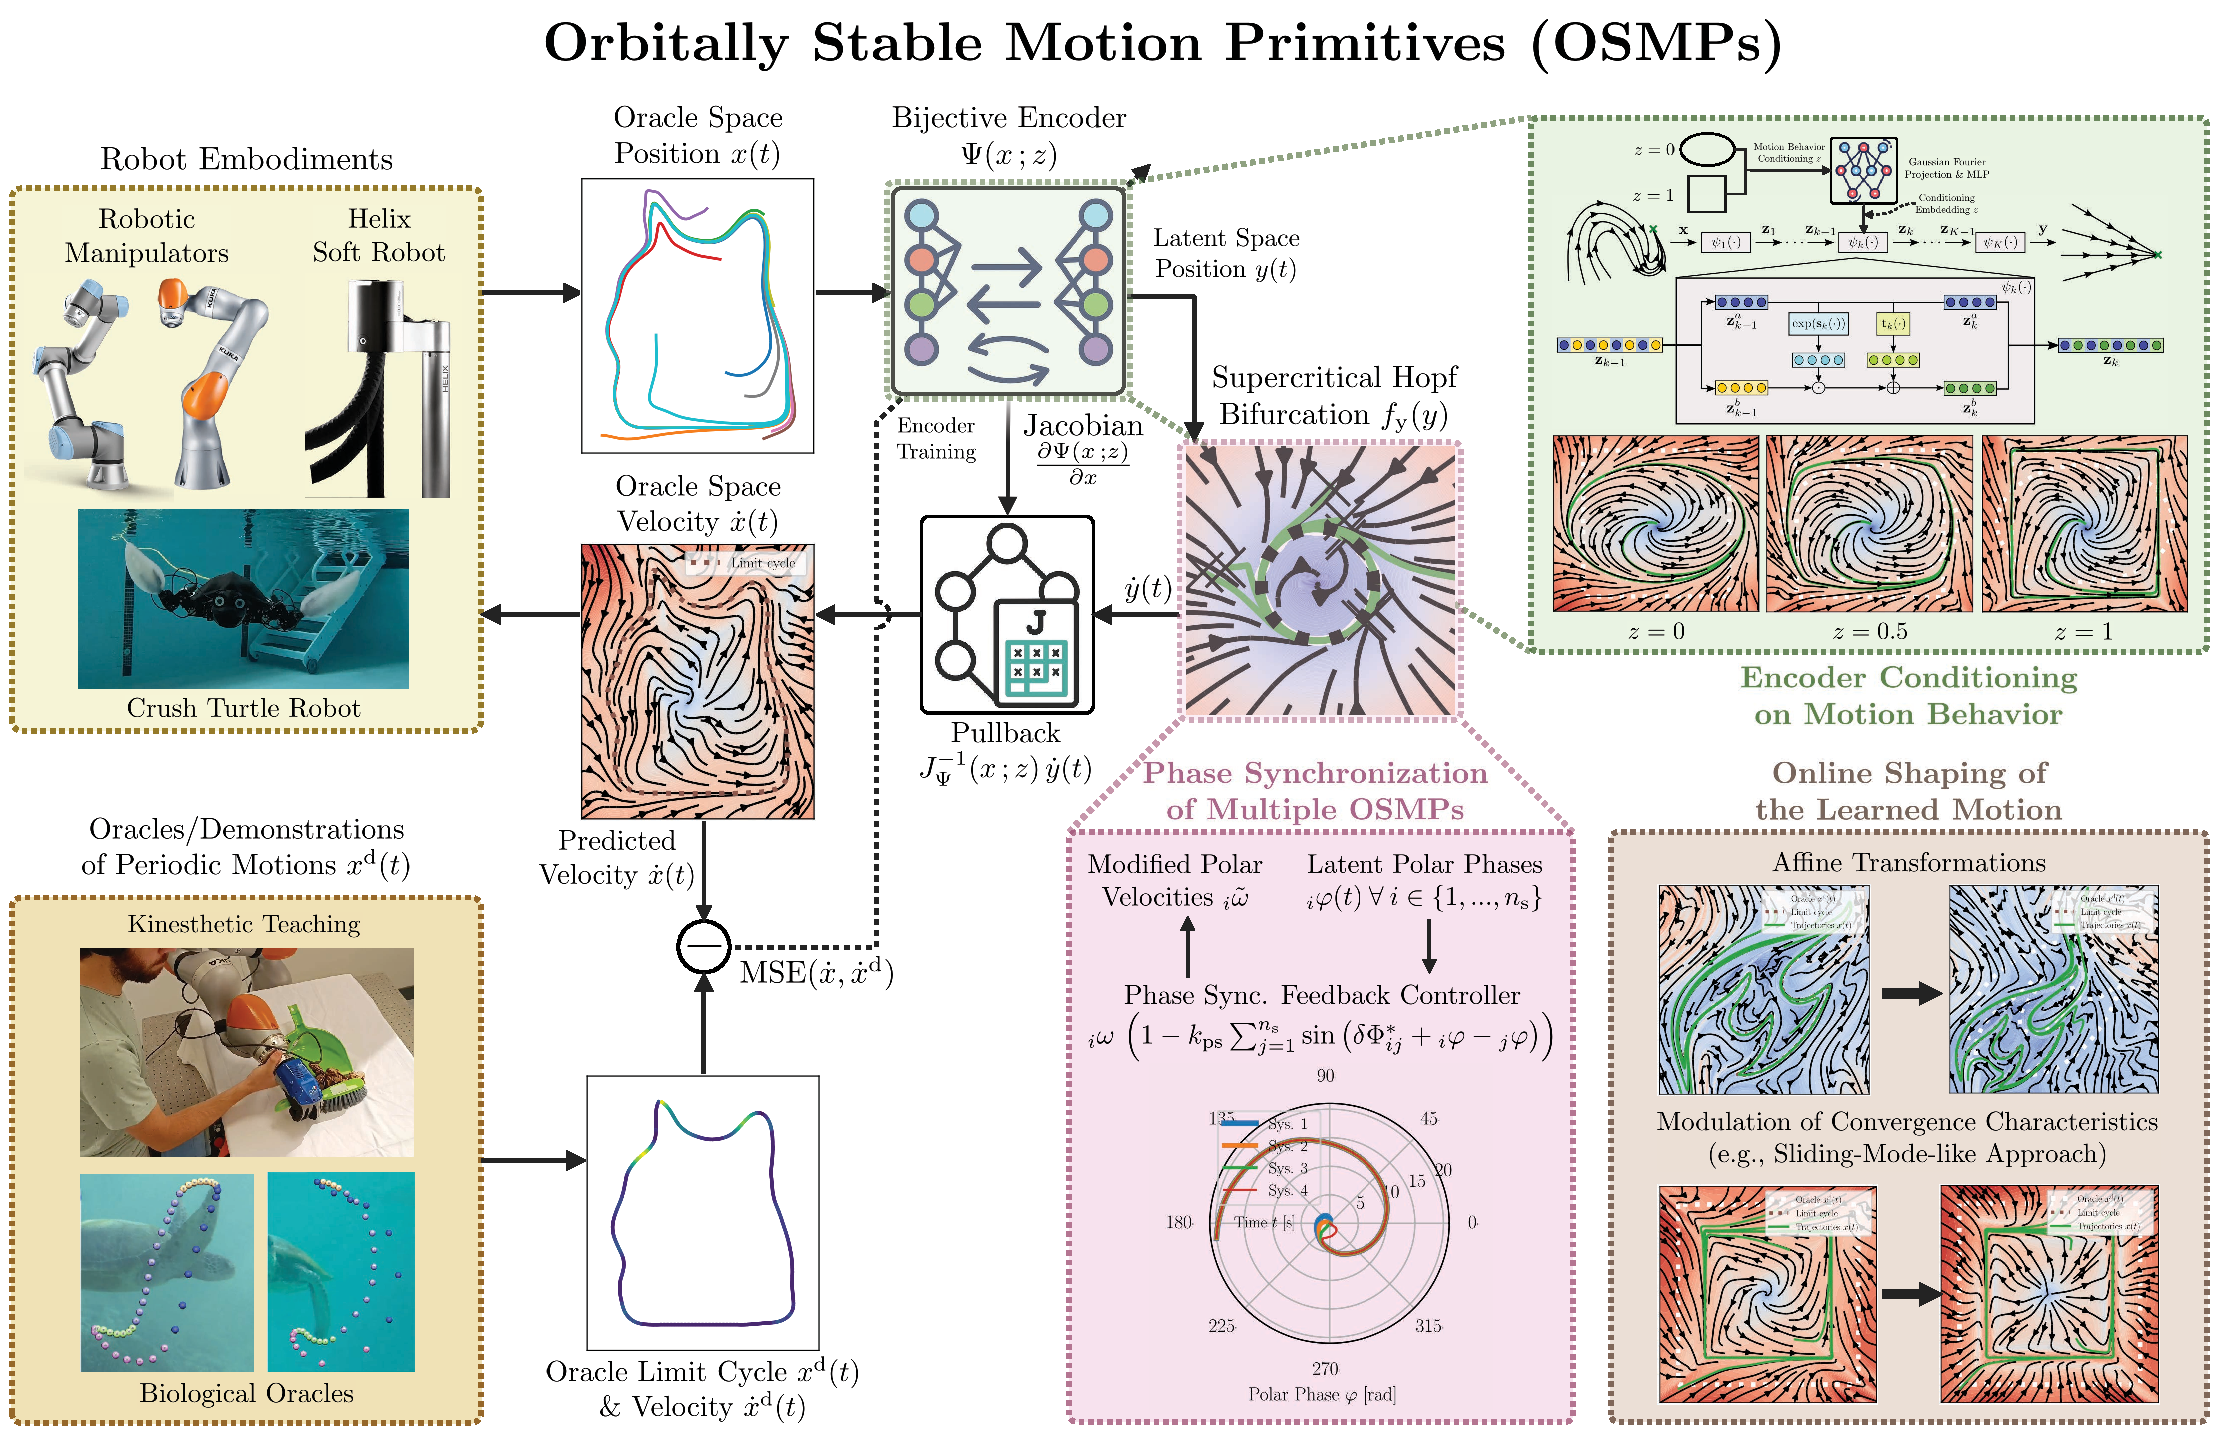
\includegraphics[width=1.0\linewidth]{osmp/figures/methodology_overview/osmp_methodology_overview_v2_compressed.pdf}
    \caption{
    \textbf{Overview of the methodology of \glsxtrfull{OSMP}:}
    Periodic motions can be learned from demonstration via a \gls{DMP} that combines a bijective encoder with latent space dynamics defined by a supercritical Hopf bifurcation. After encoding the current oracle space position of the system into latent space and predicting the latent space velocity, the pullback operator projects the velocity back into oracle space and represents a motion reference for the various robot embodiments. During training, we enforce both the predicted velocity and the exhibited limit cycle to match the demonstrations that are, for example, provided via kinesthetic teaching or based on biological oracles.
    Multiple contributions increase the practical usefulness of the proposed methods, which include a technique to synchronize multiple \glspl{OSMP} in phase, an approach to shape the learned motion online without requiring retraining via affine transformations or even modulating the convergence characteristics, and a methodology for conditioning the encoder on the oracle which allows the \gls{OSMP} to capture multiple distinct motion behaviors and even smoothly interpolate between them.
    }
    \label{fig:osmp:methodology_overview}
\end{figure}
